\section{Implementation, integration and test plan}
\label{sect:implementationintegrationandtestplan}

\subsection{6.0 Entry Criteria}
\label{subsect: entrycriteria}
Components should be tested as soon as they are released. Though, some preliminary conditions have to be satisfied before the integration plan testing shall be put into pratice.
Such preconditions are:
\begin{itemize}
    \item all of the people involved in this process must come prepared to the meetings of the peer review. This means that they have previously and carefully read the RASD and this very same document.
    \item Some of the low level modules must be avaible in order to properly test some of the components of our system. Such low level modules consists in:
        \begin{itemize}
            \item All of the DBMS must have been configured and the DBs - Shop Database, Queue Database and Account Database- possibly prefilled with fictitious data
            \item For the integration test regarding the Shop Services Subsystem, and in particular, the Shop Info Component, the Maps API should be avaible and fully usable.
            \item In order to test the part of the QR-code scanner application implemented by us, the underlaying application, the one that assures the correct unlock and lock of the turnstills, must be avaible and correctly functioning. 
            \item To proceed with the testing and integration of the Notificate User Component, which is part of the Queue Service Subsytem, the Push Api must be fully operative.
            \item To test and integrate the Account Manager Services Subsystem, the SMS Gateway should be avaible and ready to use.
        \end{itemize}
        \item In order to test a component and its interactions with other components, it must have reached a minimum level of satifistaction of its goals and functionalities. To be more precise, we will indicate the minium level of complection of each component in order for it to take part of the integration and testing plan:
        \begin{itemize}
            \item 60 \% of the Account Manager Component
            \item 60 \% of the Authorization and Authentication Engine Component
            \item 80 \% of the Ticket Generator 
            Component
            \item 90 \% of the Ticket Scheduler Component
            \item 70 \% of the Visit Component
            \item 70 \% of the LineUp Component
            \item  60 \% of the Queue Info Component
            \item  60 \% of the Analytics Component
            \item 80 \% of the Shop Info Component
            \item 70 \% of the Manage Shop Component
            \item 80 \% of all of the different Data Manager Component present in all of the subsystem
        \end{itemize}
        The different percentage of complection are due to the role of the component in the system. The most significant the features it offers are for the application, the higher the percentage is. Also the level of criticality of the algorithms implements by a component along with the level of its interconnection with other components have been considered for deciding the level of complection.
\end{itemize}


\subsection{6.1 Elements To Be Integrated}
\label{subsect: entrycriteria}
The component that must be tested and integrated can be divideed in three main categories:
-Front-end components: Qr-code Scanner Application, Web Application, Mobile Application 
-Back-end components: Queue Services Subsystem, Shop Services Subsystem, Account Management Subsystem
-External Components: Qr-code underlaying application, SMS GateWay, DBMS, Push API, Maps API

There are two kind of integration to perform. The first integration is the integration between components that are part of the same category.
In this category we can find the integration that have to be performed within the front-end components and the back-end components internally with respect to their subsystems.
The second kind of integration concerns the integration externally to their subsystems.

Front-end components and external components are indipendent from each other, while back-end components must be integrated either with front-end components and external-components.

 Due to this architecture, it is possible to partially test first each component of a category, integrate them with other components of their same category and finally integrate all of the system.

 The main integration of the back-end components with the front-end components are:

 \begin{itemize}
    \item \textbf{Mobile Application, Queue Services}
    \item \textbf{Mobile Application, Shop Services}
    \item \textbf{Mobile Application, Account Manager Services}
    \item \textbf{Mobile Application, PUSH API}
    \item \textbf{Web Application, Queue Services}
    \item \textbf{Web Application, Shop Services}
    \item \textbf{Web Application, Account Manager Services}
    \item \textbf{QR-code scanner Application, Queue Services}
 \end{itemize}

 The main integration of the back-end components with the external components are:

 \begin{itemize}
    \item \textit{Queue Services Subsystem}
    \begin{itemize}    
        \item \textbf{Queue Services, Queue DBMS}
        \item \textbf{Queue Services, PUSH API}
        \item \textbf{Queue Services, Qr-code scanner Application} ( this is inted as external to the component....)
    \end{itemize}
    \item \textit{Shop Services Subsystem}
     \begin{itemize}  
        \item \textbf{Shop Services, Shop DBMS}
        \item \textbf{Shop Services, MAPS API}
     \end{itemize}
     \item \textit{Shop Services Subsystem}
     \begin{itemize}  
        \item \textbf{Account Manager Services, Account DBMS}
     \end{itemize}  
 \end{itemize}

 \subsection{6.3 Integration Testing Strategy}
\label{subsect:integrationtestingstrategy}
According to what previously stated and concordingly with the nature of the application we are going to develop, we decided to test our system following a bottom up approach in combination with critical modules.
Thus, we decided to implement in first instance the QueueScheduler Component, which is the core module of our application, and, indeed, the most critical and delicate one. After this component is fully functional and tested, it will be possible to proceed all of the other components that some one gravitate around it with a thread-based integration. In the thread-based integration, the external dependencies will be integrated before the others: the bottom-up approach is intended this way.
This way, it will be possible to parallelize the developement phase and, moreover, to have more of an immediate feedback also at UX level. Further more, using this approach, the effort spent in providing stubs and drivers will be minimal.

In this section we will describe the order of integration of components and subsystems.
As a notation, an arrow going from a A to B means that B needs A in order to be tested, so that A needs to have been previously implemented.

\subsubsection{6.1.1 Software Integration sequence}
\label{subsect: softwareintegrationsequence}
\textbf{Queue Services}
\begin{itemize}
    \item \textbf{1.External Dependencies}
    \begin{figure}[h!]
        \centering
        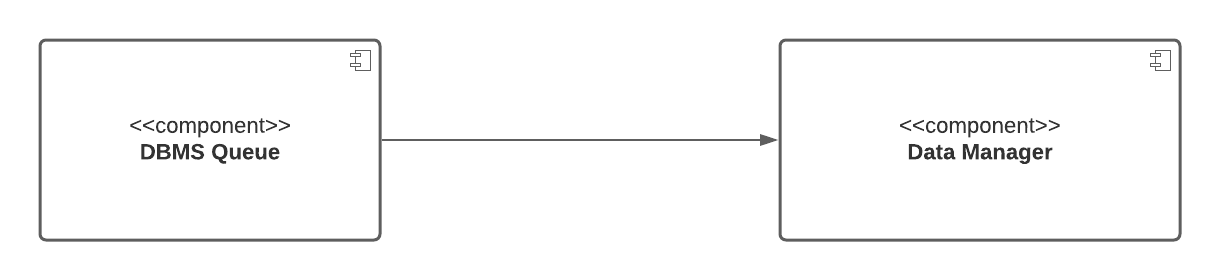
\includegraphics[width=1\textwidth]{Images/Test Diagram/Queue/ExternalDepDBMS.png}
        \caption{\label{fig:QueueExternalDepDBMS}{Queue DBMS depencency}}
    \end{figure}  
    
    \begin{figure}[h!]
        \centering
        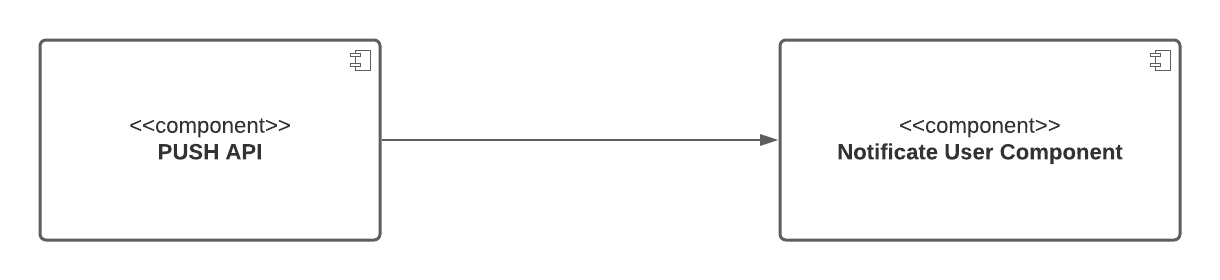
\includegraphics[width=1\textwidth]{Images/Test Diagram/Queue/ExternalDepPUSH.png}
        \caption{\label{fig:QueueExternalDepPUSH}{PUSH API depencency}}
    \end{figure}  
    
    \begin{figure}[h!]
        \centering
        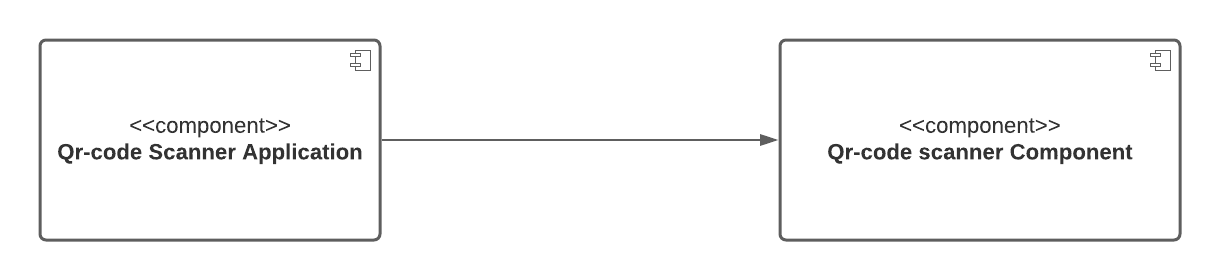
\includegraphics[width=1\textwidth]{Images/Test Diagram/Queue/ExternalDepQRCOMPO.png}
        \caption{\label{fig:QueueExternalDepQRCOMPO}{Qr-code scanner application depencency}}
    \end{figure} 
   \item \textbf{2.Internal progressive component integration}
    \begin{figure}[h!]
        \centering
        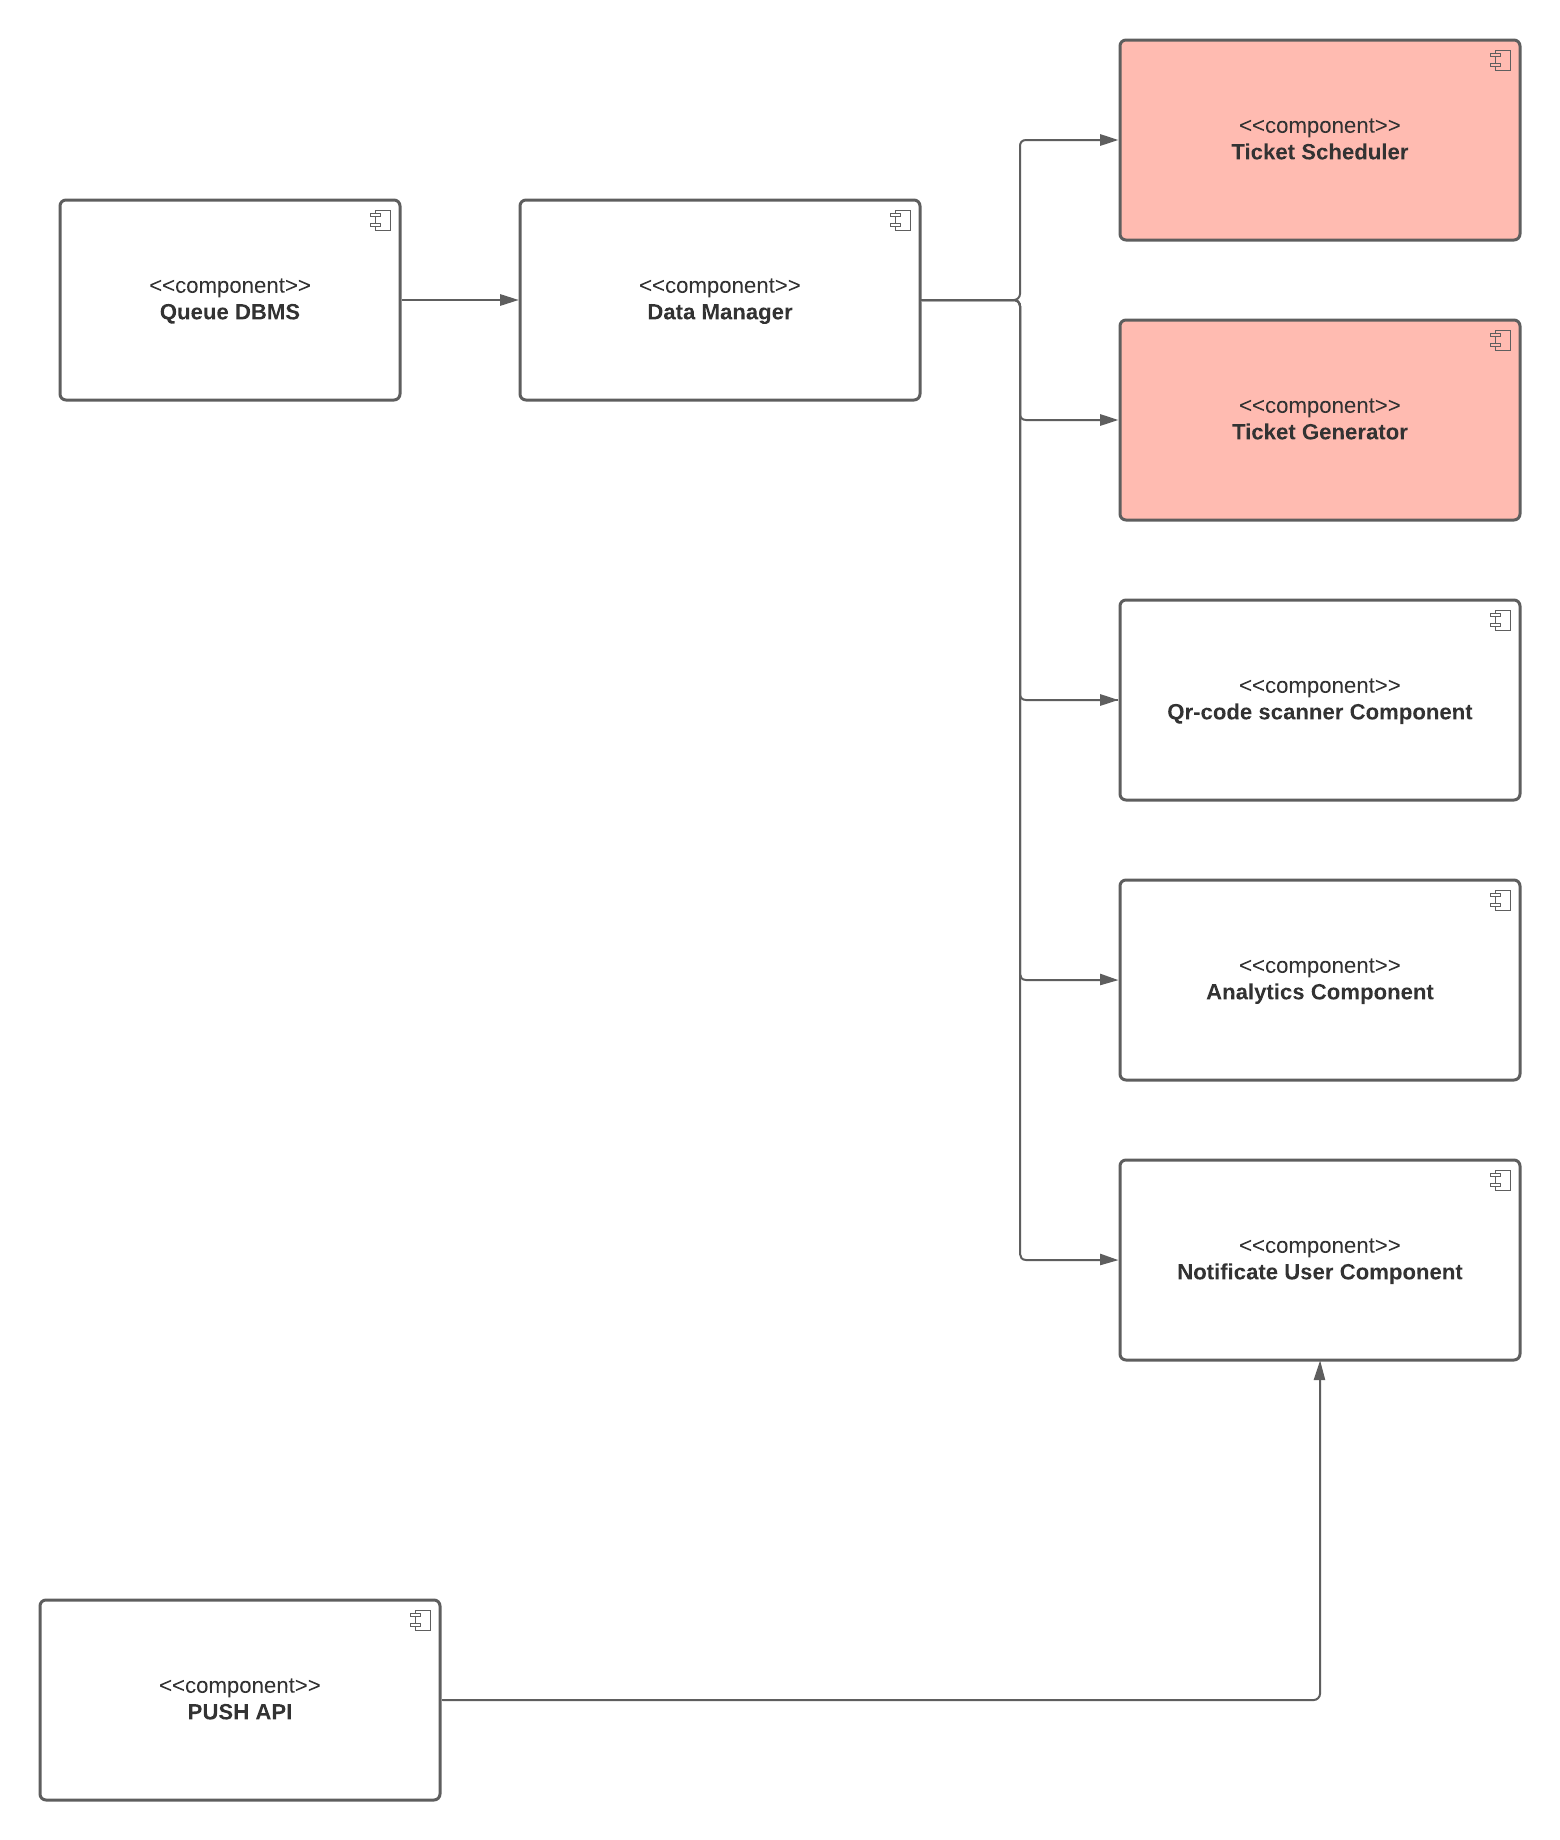
\includegraphics[width=1\textwidth]{Images/Test Diagram/Queue/queueserviceprogressive/2.0.png}
        \caption{\label{fig:QueueInternal2}{Progressive Integration 1}}
    \end{figure} 
    \begin{figure}[h!]
        \centering
        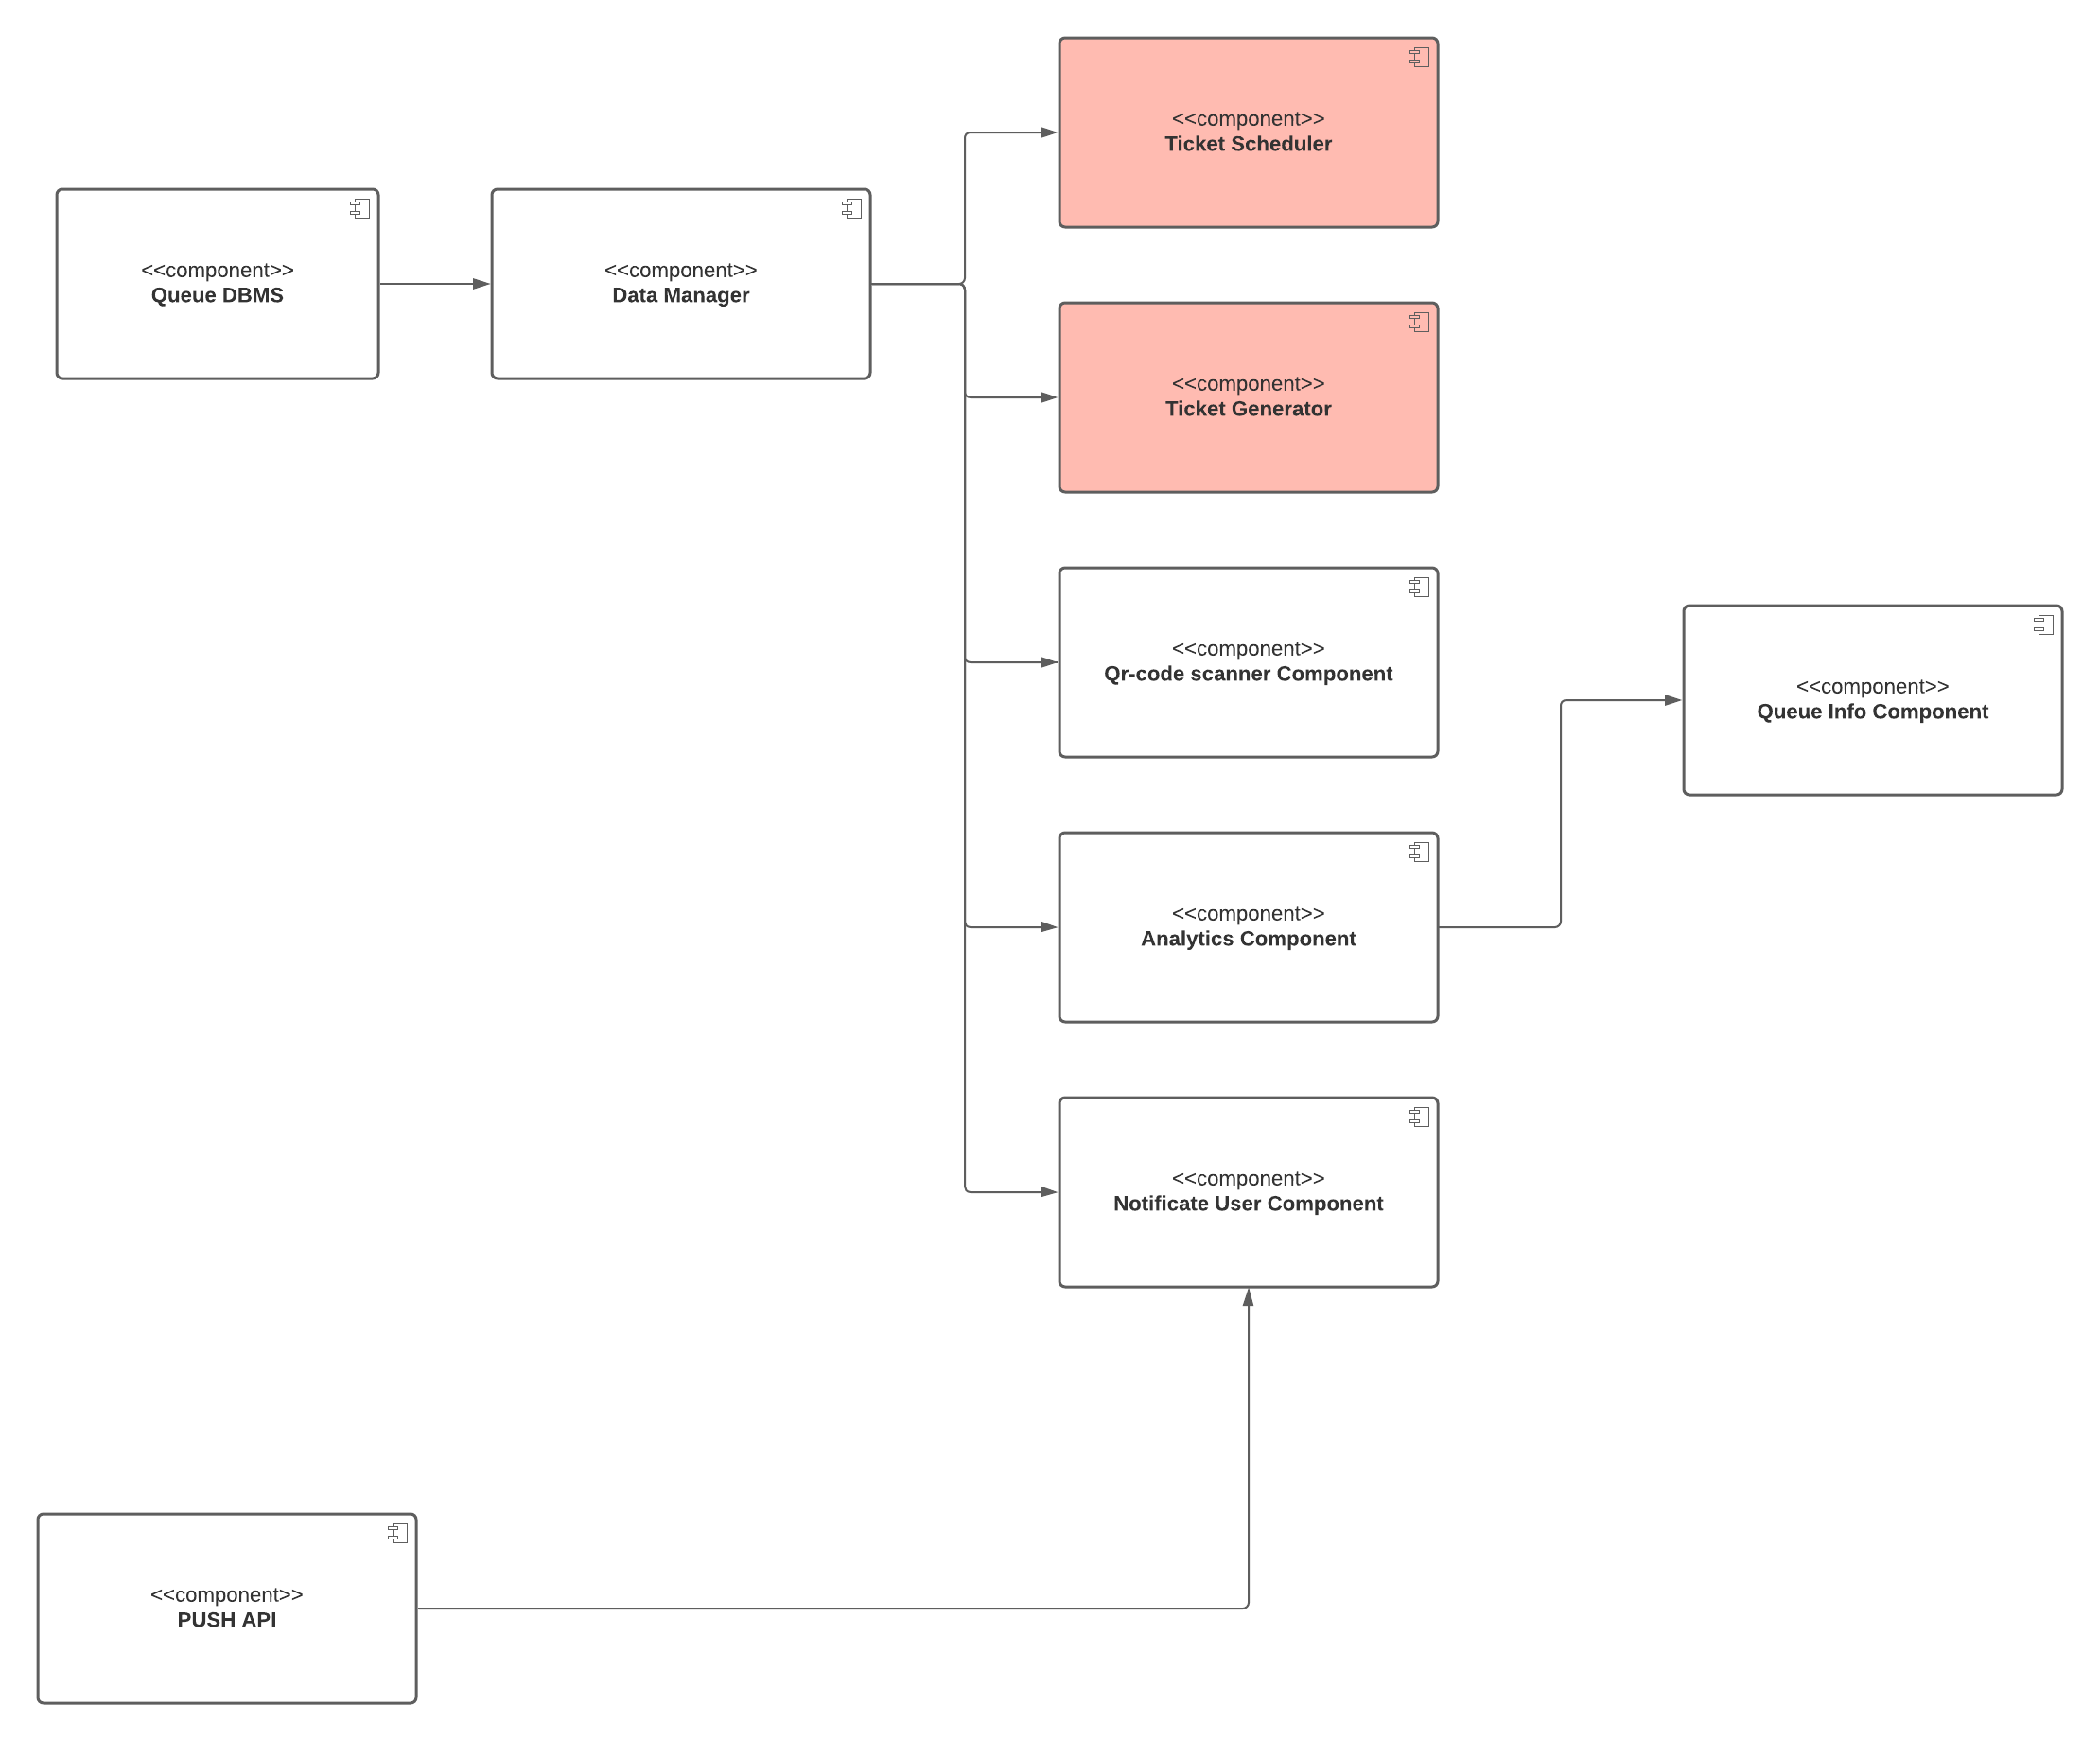
\includegraphics[width=1\textwidth]{Images/Test Diagram/Queue/queueserviceprogressive/2.1.png}
        \caption{\label{fig:QueueInternal2.1}{Progressive Integration 2}}
    \end{figure} 
    \begin{figure}[h!]
        \centering
        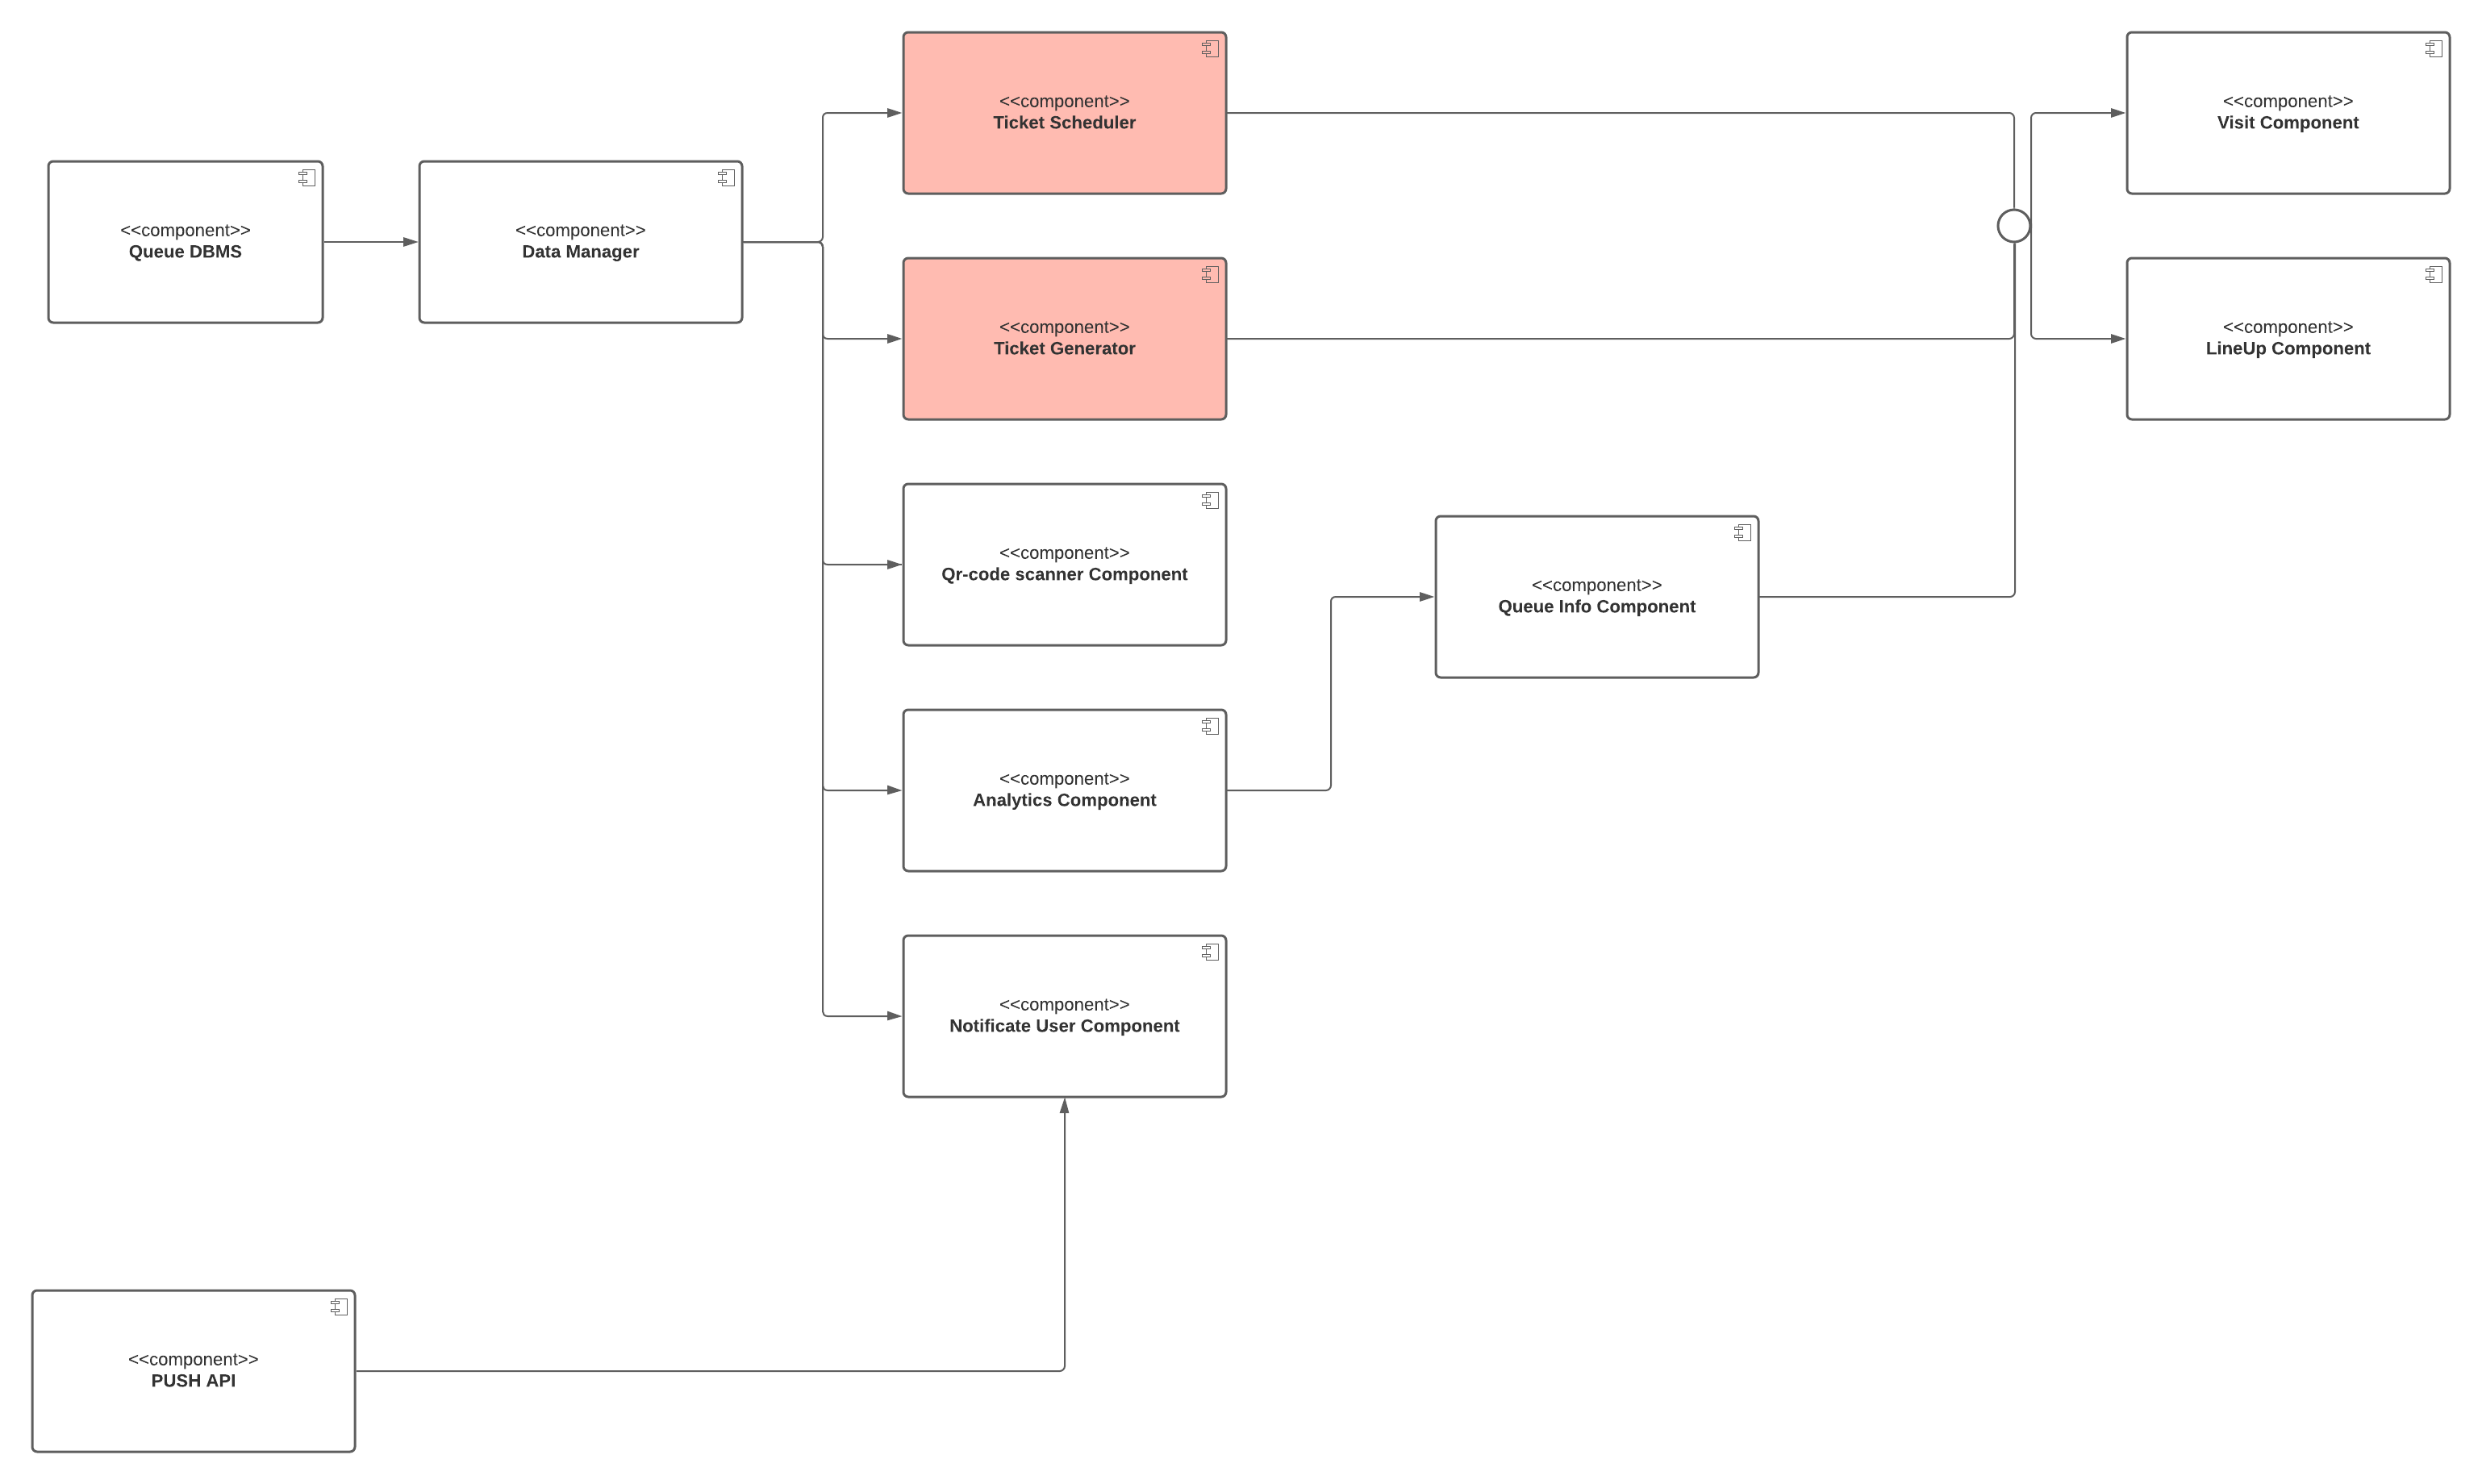
\includegraphics[width=1\textwidth]{Images/Test Diagram/Queue/queueserviceprogressive/3.png}
        \caption{\label{fig:QueueInternal3}{Progressive Integration 3}}
    \end{figure} 


    
\end{itemize}

\textbf{Shop Services}
\begin{itemize}
    \item \textbf{1.External Dependencies}
    \begin{figure}[h!]
        \centering
        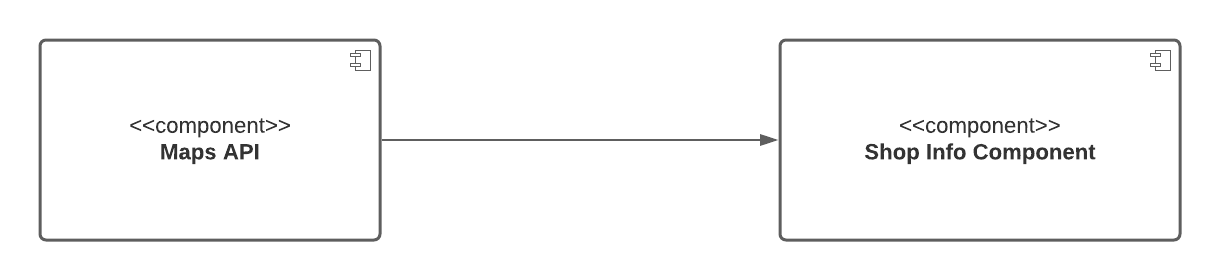
\includegraphics[width=1\textwidth]{Images/Test Diagram/Shop/maps.png}
        \caption{\label{fig:ShopExternalDepMAPS}{Maps API depencency}}
    \end{figure}  
    
    \begin{figure}[h!]
        \centering
        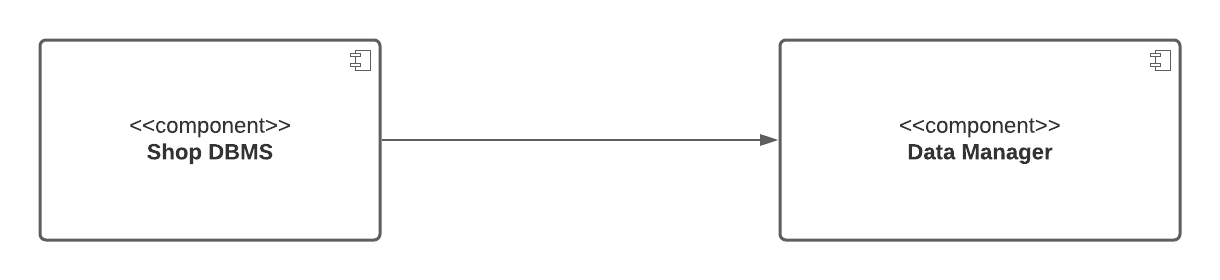
\includegraphics[width=1\textwidth]{Images/Test Diagram/Shop/data.png}
        \caption{\label{fig:ShopExternalDepDBMS}{Shop DBMS depencency}}
    \end{figure}
    \item \textbf{2.Internal progressive components integration} 
    \begin{figure}[h!]
        \centering
        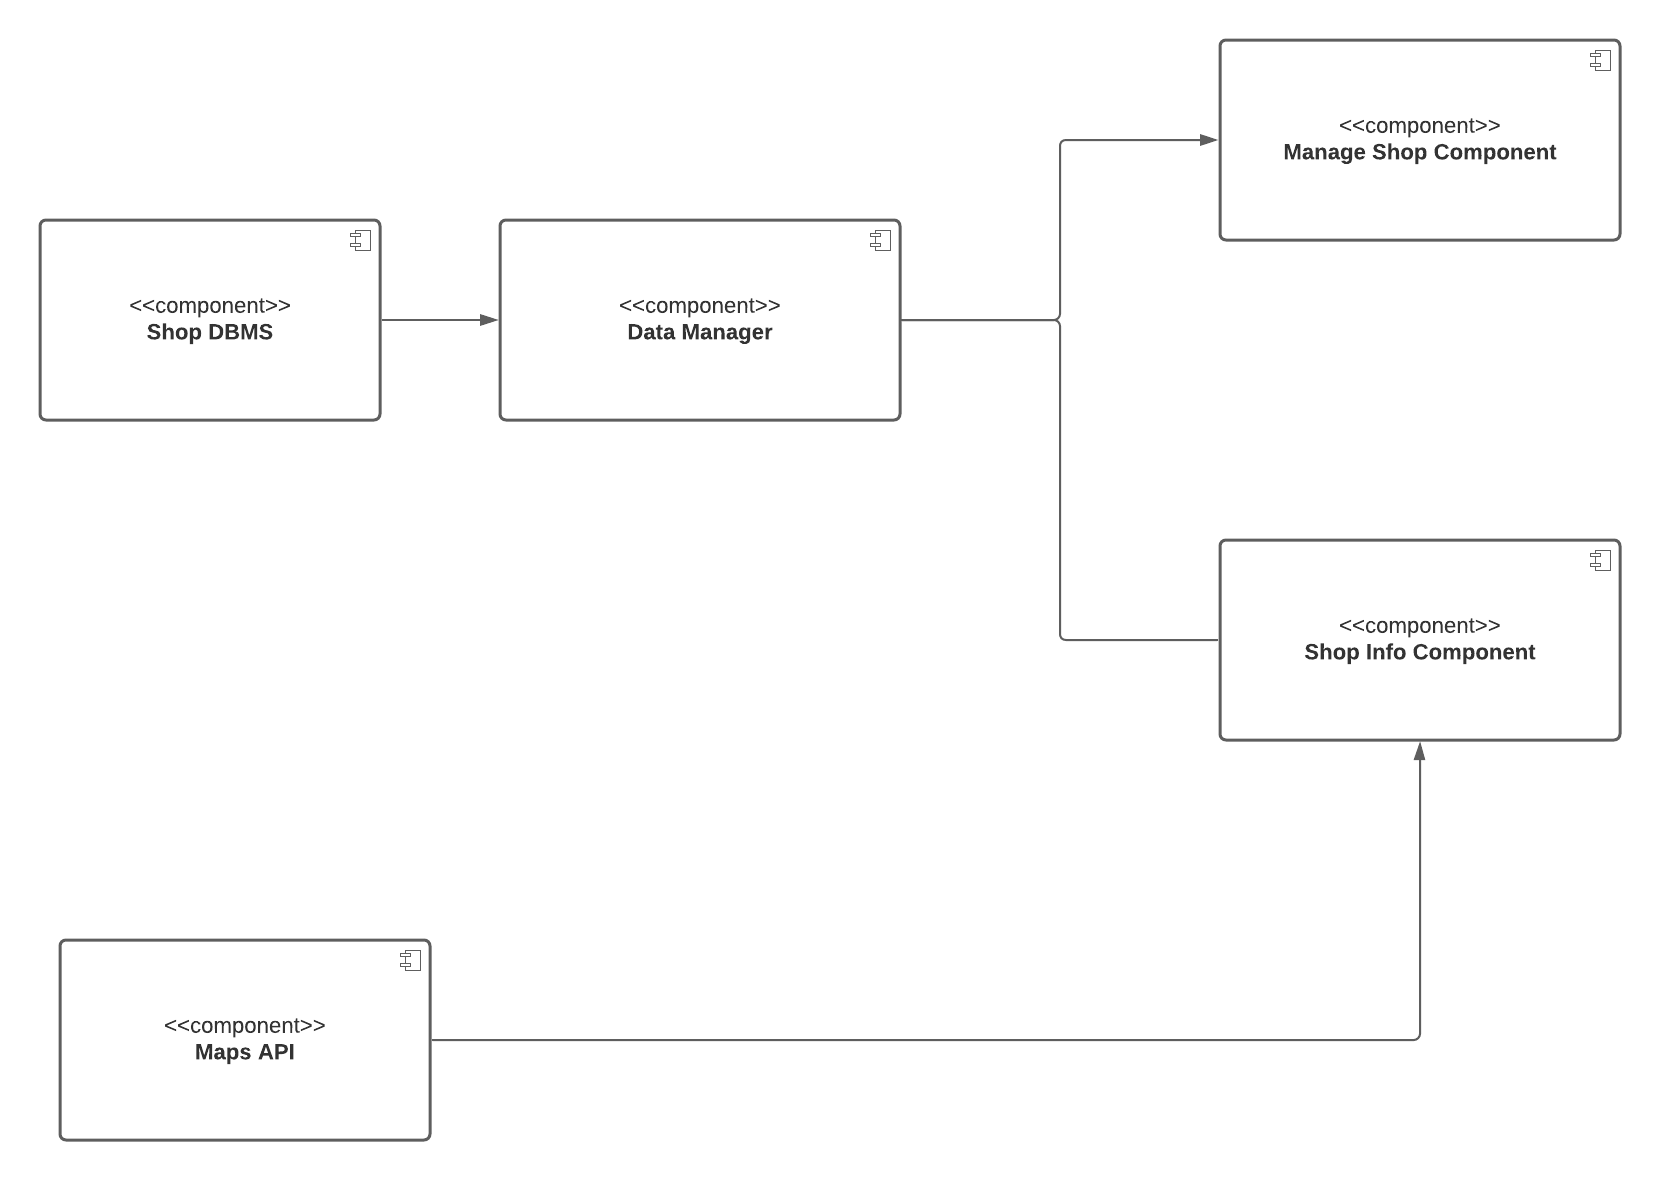
\includegraphics[width=1\textwidth]{Images/Test Diagram/Shop/2Shop (1).png}
        \caption{\label{fig:Shopinternal}{Shop Progressive 1}}
    \end{figure}  
\end{itemize}

\textbf{Account ManagerServices}
\begin{itemize}
    \item \textbf{1.External Dependencies}
    \begin{figure}[h!]
        \centering
        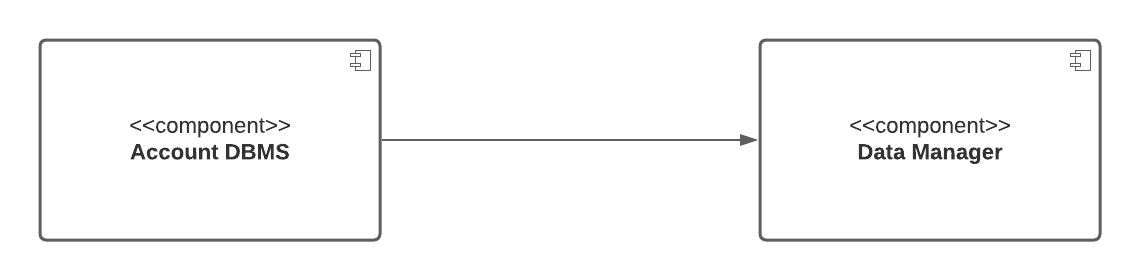
\includegraphics[width=1\textwidth]{Images/Test Diagram/Account/ExternalDependenciesDBMS.png}
        \caption{\label{fig:AccountExternalDepDBMS}{Account DBMS depencency}}
    \end{figure}  
    
    \begin{figure}[h!]
        \centering
        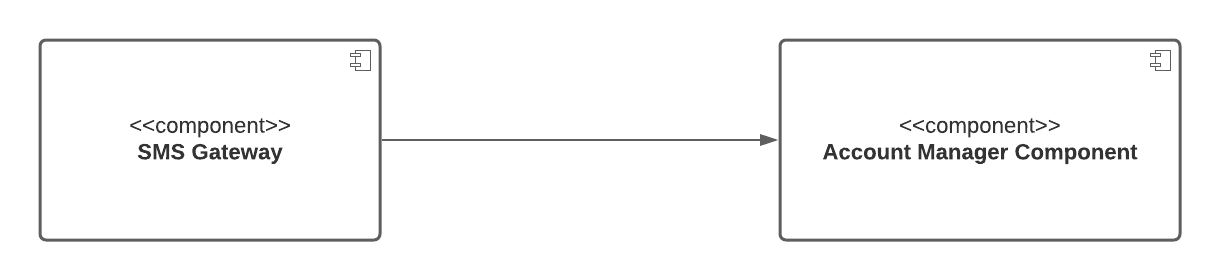
\includegraphics[width=1\textwidth]{Images/Test Diagram/Account/ExternalDependenciesSMS.png}
        \caption{\label{fig:AccountExternalDepSMS}{SMS Gateway depencency}}
    \end{figure}  
    \textbf{2.Internal progressive components integration}
    \begin{figure}[h!]
        \centering
        \includegraphics[width=1\textwidth]{Images/Test Diagram/Account/subAccount 1.png}
        \caption{\label{fig:progressiveAccount1}{progressive sequence 1}}
    \end{figure} 
    \begin{figure}[h!]
        \centering
        \includegraphics[width=1\textwidth]{Images/Test Diagram/Account/subAccount 2.png}
        \caption{\label{fig:progressiveAccount1}{progressive sequence 2}}
    \end{figure} 

\end{itemize}


\subsubsection{6.2.1 Subsystem Integration Sequence}
\label{subsect: subsytemintegrationsequence}

The following diagrams present the integration of the subsytems with the front-end components.

\begin{figure}[h!]
    \centering
    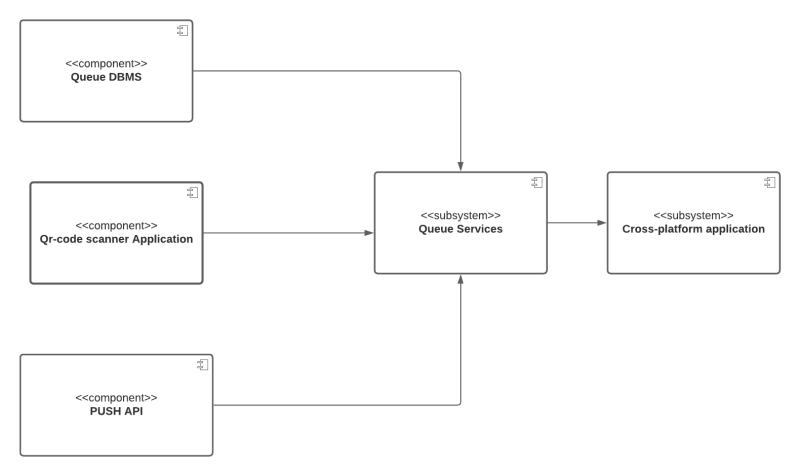
\includegraphics[width=1\textwidth]{Images/Test Diagram/view.png}
    \caption{\label{fig:viewQueue}{integration Queue Service Subsystem with front-end component}}
\end{figure} 
\begin{figure}[h!]
    \centering
    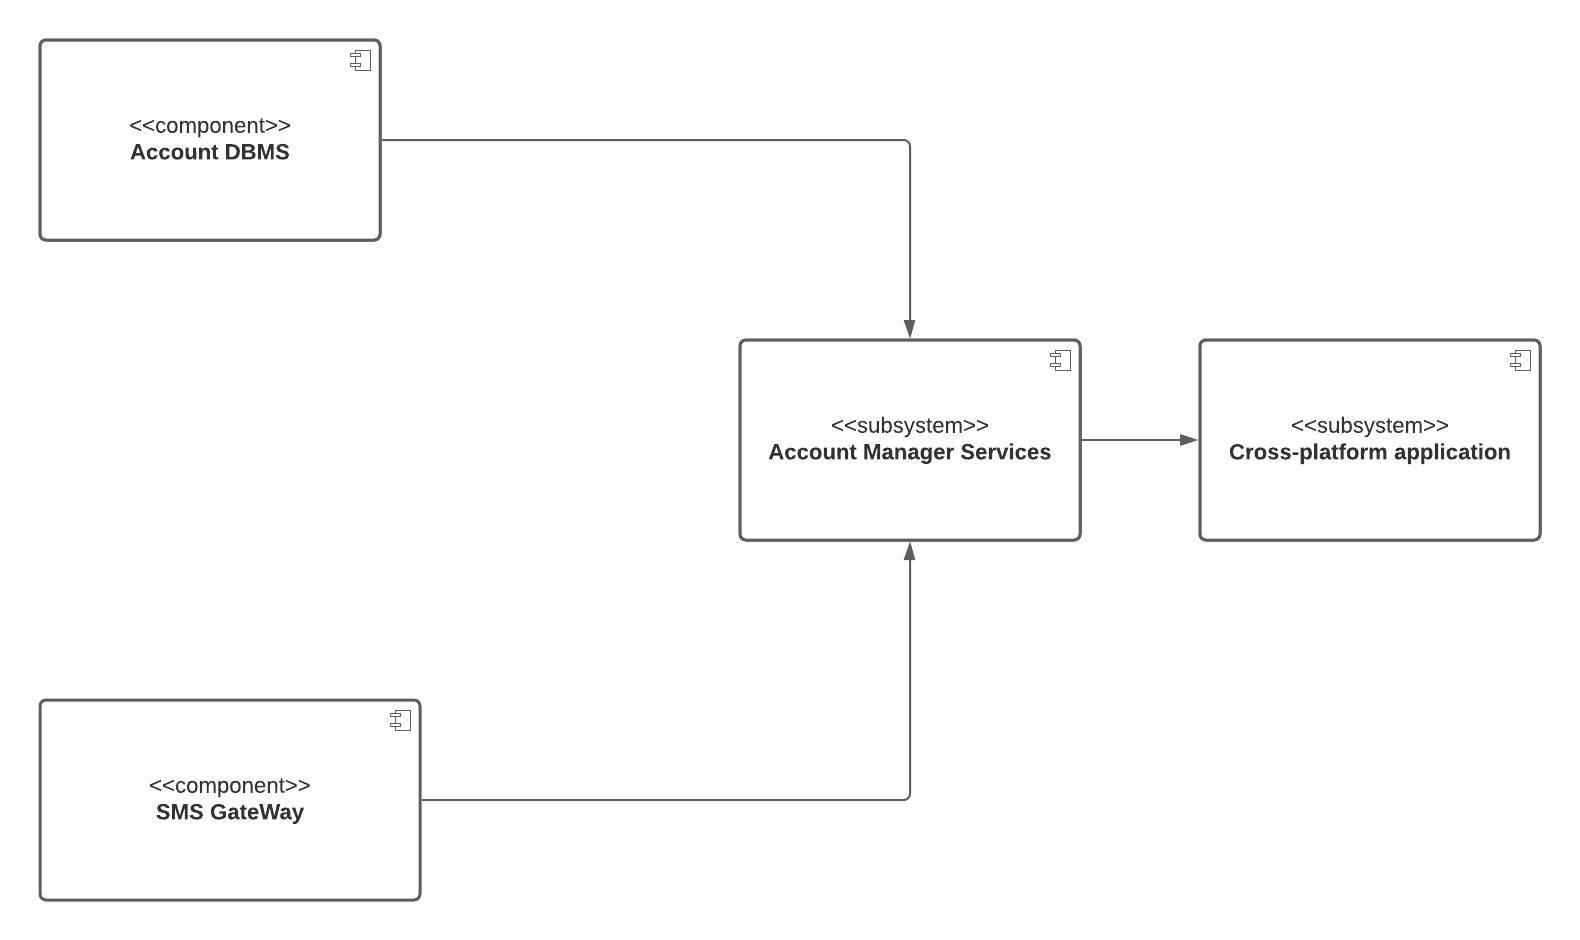
\includegraphics[width=1\textwidth]{Images/Test Diagram/viewAccount.png}
    \caption{\label{fig:viewAccount}{integration Account Manager Subsystem with front-end component}}
\end{figure} 
\begin{figure}[h!]
    \centering
    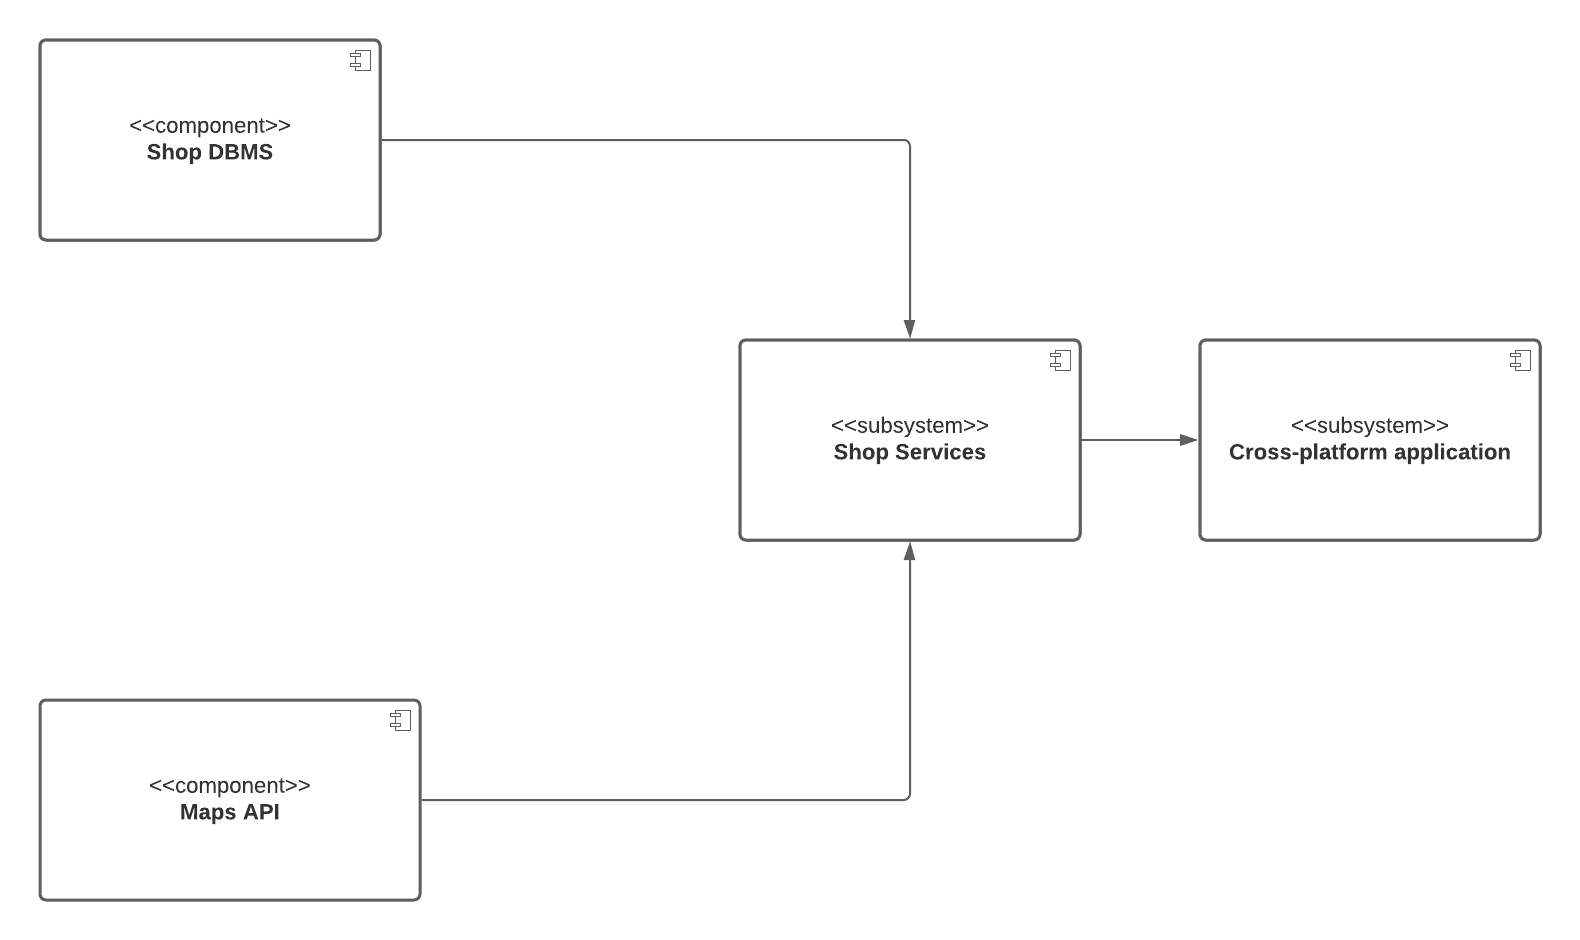
\includegraphics[width=1\textwidth]{Images/Test Diagram/viewShop.png}
    \caption{\label{fig:viewAccount}{integration Shop Services Subsystem with front-end component}}
\end{figure} 


Finally, once all of the subsystems are fully integrated, we are ready to put together, ready for deployment, the Clup Application.

\begin{figure}[h!]
    \centering
    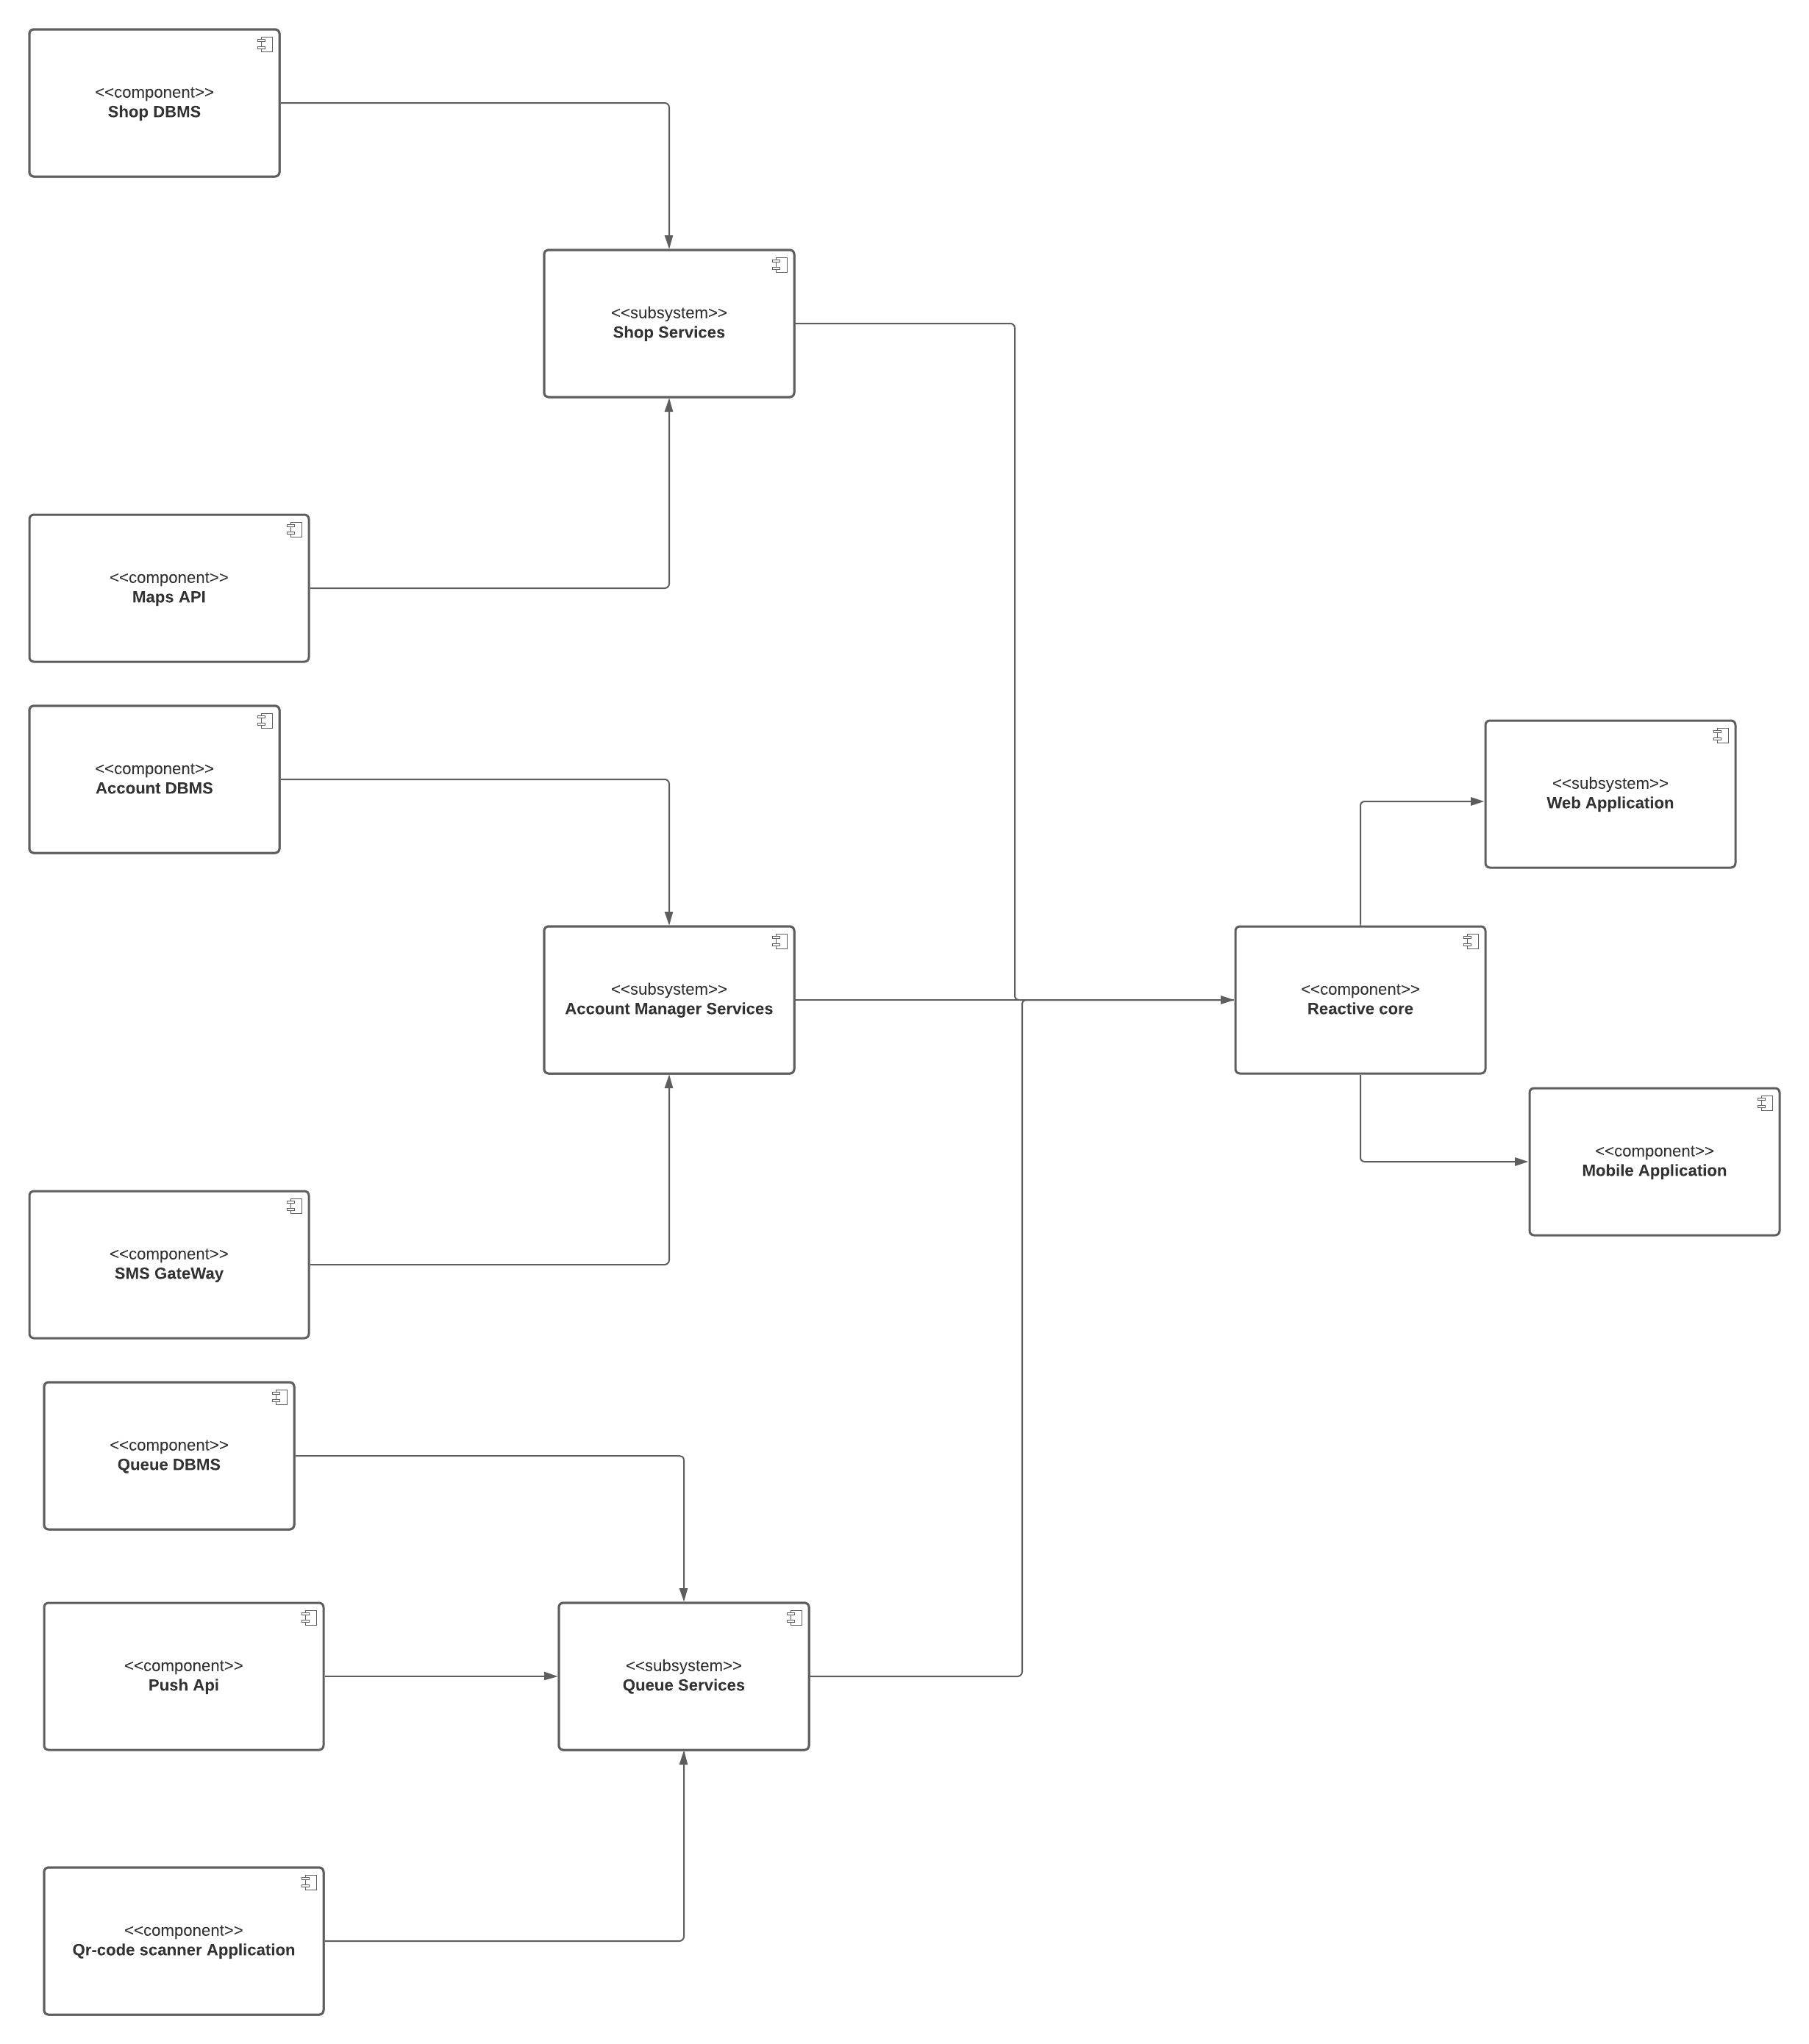
\includegraphics[width=1\textwidth]{Images/Test Diagram/whole application.png}
    \caption{\label{fig:wholeapp}{System integration}}
\end{figure} 






